%%%%%%%%%%%%%%%%%%%%%%%%%%%%%%%%%%%%%%%
% Wenneker Resume/CV
% LaTeX Template
% Version 1.1 (19/6/2016)
%
% This template has been downloaded from:
% http://www.LaTeXTemplates.com
%
% Original author:
% Frits Wenneker (http://www.howtotex.com) with extensive modifications by 
% Vel (vel@LaTeXTemplates.com)
%
% License:
% CC BY-NC-SA 3.0 (http://creativecommons.org/licenses/by-nc-sa/3.0/
%
%%%%%%%%%%%%%%%%%%%%%%%%%%%%%%%%%%%%%%

%----------------------------------------------------------------------------------------
%	PACKAGES AND OTHER DOCUMENT CONFIGURATIONS
%----------------------------------------------------------------------------------------

\documentclass[a4paper,12pt]{memoir} % Font and paper size
\usepackage{hyperref}
\usepackage{color}
\usepackage{pdfpages}
\usepackage{xcolor}
\hypersetup{
    pdftitle={},
    pdfauthor={},
    pdfsubject={},
    pdfkeywords={},
    colorlinks=false,       % no link border color
    allbordercolors=white    % white border color for all
}
\RequirePackage{xcolor}
%%%%%%%%%%%%%%%%%%%%%%%%%%%%%%%%%%%%%%%%%
% Wenneker Resume/CV
% Structure Specification File
% Version 1.1 (19/6/2016)
%
% This file has been downloaded from:
% http://www.LaTeXTemplates.com
%
% Original author:
% Frits Wenneker (http://www.howtotex.com) with extensive modifications by 
% Vel (vel@latextemplates.com)
%
% License:
% CC BY-NC-SA 3.0 (http://creativecommons.org/licenses/by-nc-sa/3.0/)
%
%%%%%%%%%%%%%%%%%%%%%%%%%%%%%%%%%%%%%%%%%

%----------------------------------------------------------------------------------------
%	PACKAGES AND OTHER DOCUMENT CONFIGURATIONS
%----------------------------------------------------------------------------------------

\usepackage{XCharter} % Use the Bitstream Charter font
\usepackage[utf8]{inputenc} % Required for inputting international characters
\usepackage[T1]{fontenc} % Output font encoding for international characters

\usepackage[top=1cm,left=1cm,right=1cm,bottom=1cm]{geometry} % Modify margins

\usepackage{graphicx} % Required for figures

\usepackage{flowfram} % Required for the multi-column layout

\usepackage{url} % URLs

\usepackage[usenames,dvipsnames]{xcolor} % Required for custom colours

\usepackage{tikz} % Required for the horizontal rule

\usepackage{enumitem} % Required for modifying lists
\setlist{noitemsep,nolistsep} % Remove spacing within and around lists

\setlength{\columnsep}{\baselineskip} % Set the spacing between columns

% Define the left frame (sidebar)
\newflowframe{0.2\textwidth}{\textheight}{0pt}{0pt}[left]
\newlength{\LeftMainSep}
\setlength{\LeftMainSep}{0.2\textwidth}
\addtolength{\LeftMainSep}{1\columnsep}
 
% Small static frame for the vertical line
\newstaticframe{1.5pt}{\textheight}{\LeftMainSep}{0pt}
 
% Content of the static frame with the vertical line
\begin{staticcontents}{1}
\hfill
\tikz{\draw[loosely dotted,color=RoyalBlue,line width=1.5pt,yshift=0](0,0) -- (0,\textheight);}
\hfill\mbox{}
\end{staticcontents}
 
% Define the right frame (main body)
\addtolength{\LeftMainSep}{1.5pt}
\addtolength{\LeftMainSep}{1\columnsep}
\newflowframe{0.7\textwidth}{\textheight}{\LeftMainSep}{0pt}[main01]

\pagestyle{empty} % Disable all page numbering

\setlength{\parindent}{0pt} % Stop paragraph indentation

%----------------------------------------------------------------------------------------
%	NEW COMMANDS
%----------------------------------------------------------------------------------------

\newcommand{\userinformation}[1]{\renewcommand{\userinformation}{#1}} % Define a new command for the CV user's information that goes into the left column

\newcommand{\cvheading}[1]{{\Huge\bfseries\color{RoyalBlue} #1} \par\vspace{.6\baselineskip}} % New command for the CV heading
\newcommand{\cvsubheading}[1]{{\Large\bfseries #1} \bigbreak} % New command for the CV subheading

\newcommand{\Sep}{\vspace{1em}} % New command for the spacing between headings
\newcommand{\SmallSep}{\vspace{0.5em}} % New command for the spacing within headings

\newcommand{\aboutme}[2]{ % New command for the about me section
\textbf{\color{RoyalBlue} #1}~~#2\par\Sep
}
	
\newcommand{\CVSection}[1]{ % New command for the headings within sections
{\Large\textbf{#1}}\par
\SmallSep % Used for spacing
}

\newcommand{\CVItem}[2]{ % New command for the item descriptions
\textbf{\color{RoyalBlue} #1}\par
#2
\SmallSep % Used for spacing
}

\newcommand{\bluebullet}{\textcolor{RoyalBlue}{$\circ$}~~} % New command for the blue bullets
 % Include the file specifying document layout and packages

%----------------------------------------------------------------------------------------
%	NAME AND CONTACT INFORMATION 
%----------------------------------------------------------------------------------------

\userinformation{ % Set the content that goes into the sidebar of each page
\begin{flushright}
% Comment out this figure block if you don't want a photo
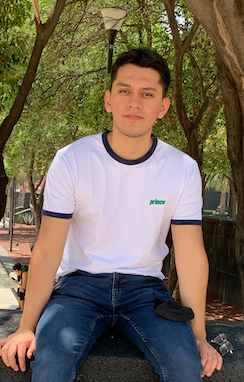
\includegraphics[width=0.9\columnwidth]{photo.jpg}\\[\baselineskip] % Your photo
\small % Smaller font size
\textbf{Luis Carranza} \\ % Your name
\textbf{\\Emails } 

\includegraphics[scale=0.03]{logos/gmail.png}
\href{mailto:lucalice76@gmail.com}{ lucalice76@gmail.com} \\ % Your email address
\href{mailto:lucalice@comunidad.unam.mx}{lucalice@
comunidad.unam.mx} \\ % Your email address

\textbf{}
\textbf{Phone } 

\includegraphics[scale=0.03]{logos/telefono.png} \\
(+52) 5561168001 \\ % Your phone number

\textbf{Telegram}

\includegraphics[scale=0.03]{logos/telegram.png} \\
\href{https://t.me/lucalice76}{https://t.me/lucalice76}\\

\textbf{LinkedIn}

\includegraphics[scale=0.03]{logos/linkedIN.png} \\
\href{https://www.linkedin.com/in/luisenrique-carranza}{www.linkedin.com/in
/luisenrique-carranza}


\textbf{Expected Graduation} \\
May-June 2022

\Sep % Some whitespace
\vfill % Whitespace under this block to push it up under the photo
\end{flushright}
}

%----------------------------------------------------------------------------------------

\begin{document}

\userinformation % Print your information in the left column

\framebreak % End of the first column

%----------------------------------------------------------------------------------------
%	HEADING
%----------------------------------------------------------------------------------------

\cvheading{Luis Enrique Carranza Escobar} % Large heading - your name

\cvsubheading{Student Computer Engineering} % Subheading - your occupation/specialization

%----------------------------------------------------------------------------------------
%	ABOUT ME
%----------------------------------------------------------------------------------------

\aboutme{About Me}{I am a student of computer engineering and I study at Faculty of Engineering of UNAM. I consider myself a learner, focused, responsible and restorative person. In addition, I enjoy solving problems mainly programming problems or related with mathematics. I like collaborating with people who have a different culture, I like learning new languages and meeting new people.
}

%----------------------------------------------------------------------------------------
%	EDUCATION
%----------------------------------------------------------------------------------------

\CVSection{Education}

%------------------------------------------------

\CVItem{2017 - Actually, Universidad Nacional Autónoma de México}{Bachelor's degree Computer Engineering}

%------------------------------------------------

\CVItem{2018 - 2021, Instituto Politécnico Nacional}{English - CELEX UPIICSA}

\CVItem{2014 - 2017, Universidad Nacional Autónoma de México}{High School - Colegio de Ciencias y Humanidades}

%------------------------------------------------

\Sep % Extra whitespace after the end of a major section

%----------------------------------------------------------------------------------------
%	EXPERIENCE
%----------------------------------------------------------------------------------------

\CVSection{Extracurricular Activities}

%------------------------------------------------

\CVItem{September 2020, \textit{Hackathon}, AWS}{
Detailed Achievements:
\begin{itemize}
	\item Basic use of \textsc{AWS (Amazon Web Services)}:
	\item Basic Web Design  
	\begin{itemize}
		\item HTML5
		\item CSS3
		\item JavaScript
		\item Responsive Web Design
	\end{itemize}
\end{itemize}
}

\CVItem{February 2021 - August 2021, \textit{CISCO Certification Program }, CCNA Enterprise}{
Detailed Achievements:
\begin{itemize}
	\item Introduction to Networks \textsc{(ITN)}:
	\item Switching, Routing and Wireless Essentials (SRWE)
	\item Enterprise Networking, Security and Automation (ENSA)
	\item CISCO hardware configuration
	\begin{itemize}
		\item Host
		\item Servers
		\item Routers
		\item Switches
	\end{itemize}
	\item Protocols
	\item Administration of networks
\end{itemize}
}

\CVItem{August 2021, \textit{Hackathon}, Innovaccion}{
Detailed Achievements:
\begin{itemize}
	\item Basic use of \textsc{Microsoft Azure}:
	\item Azure services  
	\item Cloud services 
	\item Cloud concepts
\end{itemize}
}
%------------------------------------------------

%------------------------------------------------

\Sep % Extra whitespace after the end of a major section

%I have to use clearpage, userinformation and framebreak to creat a new page on my CV
\clearpage % Start a new page

\userinformation % Print your information in the left column

\framebreak % End of the first column
%----------------------------------------------------------------------------------------
%	COMMUNICATION SKILLS
%----------------------------------------------------------------------------------------

\CVSection{Communication Skills}

%------------------------------------------------
\CVItem{June 2018 - May 2021, \textit{CELEX UPIICSA}}{I had been studying at CELEX UPIICSA for 3 years to improve my speaking, listening and writing skills. I really love talking in English with other people.}

\CVItem{June 2020 - Mayo 2021, \textit{Conversation Club UPIICSA}}{I worked with people from other countries in a conversation club.}



%------------------------------------------------

%------------------------------------------------

\Sep % Extra whitespace after the end of a major section

%----------------------------------------------------------------------------------------
%	SKILLS
%----------------------------------------------------------------------------------------

\CVSection{Software Development Skills}

%------------------------------------------------

\CVItem{Programming}
{\begin{tabular}{p{0.2\textwidth} p{0.2\textwidth} p{0.2\textwidth}}
\bluebullet Java &  \bluebullet Swift & \bluebullet Python\\
\bluebullet C/C++ & \bluebullet SQL & \bluebullet VHDL & \bluebullet JavaScript\\
\end{tabular}}

%------------------------------------------------

\CVItem{Computer Software}
{\begin{tabular}{p{0.2\textwidth} p{0.2\textwidth} p{0.2\textwidth}}
 \bluebullet Linux &  \bluebullet macOS & \bluebullet Windows & \bluebullet Xcode & \bluebullet Visual Studio Code & \bluebullet Terminal & \bluebullet Windows CMD & \bluebullet SQL Server\\
\end{tabular}}

%------------------------------------------------

\Sep % Extra whitespace after the end of a major section

%----------------------------------------------------------------------------------------
%	NEW PAGE DELIMITER
%	Place this block wherever you would like the content of your CV to go onto the next page
%----------------------------------------------------------------------------------------



%----------------------------------------------------------------------------------------
%	AWARDS
%----------------------------------------------------------------------------------------

%\CVSection{Awards}

%------------------------------------------------

%\CVItem{2010, \textit{Postgraduate Scholarship}, Cornell University}{Awarded to the top student in their final year of a Bachelors degree.}

%------------------------------------------------

\Sep % Extra whitespace after the end of a major section

%----------------------------------------------------------------------------------------
%	INTERESTS
%----------------------------------------------------------------------------------------

\CVSection{Interests}

%------------------------------------------------

\CVItem{Professionals}{Mobile Development, big data, IA, WEB design, WEB development, software design, algorithms, Networks, Data Bases}

%------------------------------------------------

\CVItem{Personal}{Guitar, singing, football soccer, finances, workout}

%------------------------------------------------

\Sep % Extra whitespace after the end of a major section

%----------------------------------------------------------------------------------------

\end{document}
